%ब
\chapter{Proposed Solutions} \label{c:solutions}

This chapter describes the four  solutions proposed to implement referential
integrity constraints in a cloud \ac{NoSQL} database system.
Section~\ref{} describes some typical ways of storing  data
dependency information in \acp{DBMS}. Section~\ref{s:metadata} desribes how
metadata is used for maintaining referential integrity in the proposed
solutions. Section\ref{s:api} describes the design of the API devloped to
implement these constraints. Section~\ref{s:baseline} presents a baseline of
the \ac{API} without any referential integrity constraints
.


\section{Introduction}

As mentioned in the previous chapters, cloud \ac{NoSQL} database systems lack
referential integrity constraints that are imposed in traditional \acp{RDBMS} to
maintain data integrity. In \acp{DBMS}, data integrity is maintained by
correctly preserving the data dependencies existing between data entities within
a database.

Most popular traditional \acp{DBMS} do so by saving such dependency information
in their \texttt{SYSTEM} tables. This can be seen in porpular \acp{DBMS} like
Oracle, PostgreSQL, MS SQL Server etc. For example, in MS SQL Server 2000, there
exists \texttt{System} tables for every database that store various details of
constraints existing within the database. The \texttt{System} table
\texttt{sysforeignkeys} stores the information for all the foreign keys existing
in the tables in a database, like the objectIDs of the table with the constraint,
IDs of the referenced and referencing columns etc. This table is looked up
whenever referential integrity checks are triggered. \citep{sys:msdn}.
Similarly, in PostgreSQL, such information is saved as views which contain the
object dependency information for a database. The view
\texttt{table\_constraints} contains the information for all the constraints in
a table belonging to the current user.% \cite{}.
The information about the constraints within a database or a table that is
stored in such tables is the metadata information. Metadata is explained in
 Section~\ref{s:cloud-databases}  

To understand how a cloud \ac{NoSQL} database system works and to deploy
the proposed solutions, the cloud \ac{NoSQL} database system Cassandra
is explored. The details of \texttt{Cassandra} is explained in
Section~\ref{s:cassandra}.

% 


As mentioned before, these proposed solutions involve using metadata in
different ways to impose referential integrity constraints in Cassandra. The
following section describes metadata briefly. This 


\section{Metadata}\label{s:metadata}
DBSs today tend to be large with respect to size or in terms of their
distribution across a network. Large-scale DBSs as well as large distributed
DBSs tend to also store and maintain metadata. Metadata generally is described
as ``Data about data''. Most of the literature talks about application
information, location information, directory hierarchy or access permissions as
the metadata that would be associated with the real data (Lin Xia et al. 2009;
Duval et al. 2002; Huang Bin \& Peng Yuxing 2010; Hackl et al. 2010; Jan-Jan Wu
et al. 2010). But in addressing the current problem of RI in NoSQL DBSs,
thepotential solutions consider storing information about dependencies or
relationships between the data entities as metadata. This metdata could then be
stored as a table(s).

In (Hackl et al. 2010) metedata management is discussed where emphasis is laid
on the synchornous updates of metadata storage. While this paper focuses on
metedata management, an interesting approach is adopted in a key-value DBS as a
part of their experiment. Metedata is managed in TokyoCabinet by inserting the
metadata in the value field, separated with semicolons (Hackl et al. 2010)

For creating metadata tables like the one shown above, it would be necessary to
derive the dependency information from the ER designs of the database. The
dependencies could then be inserted into the metadata tables using the
MetaDriver low-level API, which is described below.
 would be a reserved keyword or identifier to distinguish the
tables as metadata tables from other tables or ColumnFamilies. Since these
metadata tables could be stored on different server nodes as a part of the MDS
cluster, it might be necessary to give the metadata tables a unique name too.
For this purpose such metadata tables could have the names of their respective
databases prefixed to the '' keyword, like 'StudentMDCONSTRAINT'
as shown in Figure 6. For example, if the metadata table is designed for a
hospital DBS, it could be named as '', which would help
the MetaDriver API identify it as the metadata table belonging to the Hospital
DBS. Such a unique identifier is needed due to the distributed nature of the MDS
cluster. (Please note: The protocols needed for such an MDS cluster would be
discussed in following reports.) When an application using a NoSQL database
interacts with the database to perform any operation on the data like inserting
or updating or deleting data etc., the application normally talks to the
database engine or database driver. In NoSQL databases, this is commonly done by
the APIs the NoSQL DBMS provides, for example Thrift in Cassandra, JDO in Google
AppEngine etc. The proposed solution is an API, called MetaDriver, would be a
layer on top of such APIs. This is shown in Figure 7.

In the proposed solution, the value could include metadata about what table or
what foreign value the value of a key-value pair would refer to. Here, the
foregn value is similar to the foreign keys in RDBMSs, except that the foreign
value is not the unique primary key

In the case of NoSQL DBSs, this could mean that every replicated copy holds the
same metedata information in the value field. So values that refer to other
values in different tables could be maintained.

\section{The API and Database Schema/Model}\label{s:api}

To perform data operations like insert, update, delete, retrieve data
etc.,Cassandra provides an \acp{API} to its users. The Thrift API can support
many programming languages, making it easy for most applications to store data in
Cassandra (Gunda, 2010). For the proposed solutions, Hector, an \acp{API}
designed to work above the Thrift \acp{API} is implemented.--(\todo{Hector
details})-- This helped develop the solutions faster due to its simplicity and
efficiency in communication with Thrift \ac{API}.

The proposed solutions are writted in Java and run on a cluster
of nodes within the university's computer network. During the development a
cluster of 5 nodes were used and for testing this was increased to
(\todo{node\#}).

Pseudocodes give an informal and a high-level description of an algorithm
without using variable declarations, function calls or complicated data flows
and replaces these with simple English sentences (Wikipedia 2011). Since the
current purpose is simply to understand the key principles and steps involved in
the proposed solution, pseudocodes are the best way to describe all this without
using any conventional programming syntax. For the sake of simplicity, in the
following pseudocodes any kind of database operation is termed as request and
the metadata table is assumed to be similar to 'StudentMDCONSTRAINT' in Figure
6

The API inserts data into the column families from CSV files. The Students and
Courses details are inserted without performing any insertion checks. On the
other hand, the Enrolment column family would have referenced columns from other
column families. So it was required that checks be made prior to insertion, to
ensure that the referenced values were actually existing in the referenced
column families. For example, when the following row is to be inserted into
Enrolment some checks would have to be made to ensure data consistency and
integrity

Generally, the referential integrity constraint needs to hold whenever any data
operation is performed on the data. Referential Integrity (RI) checks are
performed each time an update operation is invoked on any entity like Student or
Course or Enrolment. As previously mentioned, the dependency information for all
entities is saved as metadata and for each solution this metadata is saved in a
different way. But for all the solutions, the RI checks for an update operation
are similar.
In an update operation there are two different types of RI checks performed,
depending on the entity that is being updated. Update RI checks for a parent
entity are different from the update RI checks for a child entity. Also, the
update operations are different depending on the 'DeleteRule'.
A parent entity contains the key that is referenced by another entity, i.e.,
child entity. Therefore, the child entity is the one with the referencing key or
the foreign key. For example, the entities Student and Course are parent
entities, while Enrolment is a child entity.Whether data is being inserted,
updated or deleted, referential integrity has to be adhered to. The actions and
the checks to be performed for each of such operations are described below.

\begin{description}
  \item  [Insert :]%An insert operation would trigger a referential integrity
%   validation when data is being inserted into a referencing table, i.e., the child table. In
% such an event, prior to entering the values in the referencing table, it is
% checked if the referencing keys exist in the referenced table. For example, when
% the enrolment details of a student are being inserted into the Enrolment table,
% a check is triggered to verify whether the StudentID exists in the Student
% table. Similarly, it is also verified that the CourseID exists in the Course
% table. If the referencing keys do not exist in the referenced tables, then the
% insert operation is not allowed. 
Prior to inserting this row, insertion checks would be made to ensure
that the SID exists in the Student Column family of the keyspace University. This piece
of information can be retrieved from the second part of the metadata
information. This is applicable to all solutions, as metadata information is
consistent across all solutions. Similarly, the Course column family would have
to be checked to ensure that SWEN100 exists. If these checks are not
implemented, then it is possible that any wrong information can be inserted and
the referential integrity constraint be violated. For example, SWEN100 may not
actually exist in Course, but without any checks it could be inserted into the
database.

Such insertion checks are introduced into all the solutions within the API.

 \item  [Update :]%When data is being updated either in the referencing table or
% the referenced table, a referential integrity validation is needed. When any
% referenced key (primary or unique) is being updated in the referenced table,
% then it has to be verified whether this key is a foreign key in any of the
% referencing tables. If a dependency is found to exist, then the applicable
% referential integrity rule is checked. So if it is a Cascade, then the
% associated foreign keys in the referencing table are updated prior to updating
% the key in the referenced table. If the rule is "Set to NULL" or "Set to
% default" then the associated foreign keys in the referencing table are set to
% NULL or default values. A Restrict would prevent the update action in the
% referenced table. 
% 
% When any foreign key is being updated in a referencing table, then a referential
% integrity validation has to be performed. It has to be ensured that the new
% updated value exists as a key in the referenced table. For example, in the
% Enrolment table, if the course details of a student (i.e. foreign key CourseID)
% are being updated to a new value, then it has to be verified that the new value
% is an existing key in the Course table. Otherwise, if the new value does not
% exist, then the update is not allowed generally.

When an update is made to a value in a column family, checks have to
be made ensuring that these changes or updates do not violate referential
integrity. Update actions would overwrite data and if such actions overwrite
values that have dependencies on them, it could lead to poor integrity. The API
would first check if the value that is being updated exists in the metadata
information as a Primary key or as a foreign key. If it is a part of the
metadata information, implying that a constraint exists on this value, then the
update would be prevented from execution and an exception would be raised.
A different kind of Update is the Upsert, where the values would be inserted if
the values to be updated do not exist already. Here, the API would check if
there are any foreign keys being inserted and would check to see if they exist
in the mentioned keyspace prior to executing the Upsert operation.
\begin{itemize}
\item Updating a parent entity: When a parent entity is being updated, its
metadata information is checked to find out its 'DeleteRule'. 'DeleteRule' for an entity
could be 'NODELETE' or 'CASCADE' and is applicable for both delete and update
operations. If the 'DeleteRule' is 'NODELETE', then the update of the entity is
not allowed. For example, in the current API, Course entities have a 'NODELETE'
rule in their metadata while the Student entities have a 'CASCADE' rule. Hence,
when a request is made to update a Course, it is not allowed by the API and an
exception is thrown. Despite this, a further check is made to see if the entity
has any child dependencies existing or not. In this dependency check, if the
entity is found to have no dependencies, the update is allowed.  For example, if
a Course entity is found to have no students enrolled for it in Enrolment, the
update operation is allowed and the Course is updated with the new value.

If the 'DeleteRule' is 'CASCADE', then the metadata is checked to identify the
referencing column families. The existence of the record marked for update in
these referencing column families is verified. If existing, the child records
are updated with the new value. Then the values in the parent entity are updated
with the new value. For example, if an update operation is invoked in the
Student column family, to change 'StudentID' '111' to '222', and its
'DeleteRule' is 'CASCADE', then the referencing column family, Enrolment is
identified using the metadata. In Enrolment, all the existing values for the
foreign key '111' are replaced with '222'. Then the 'StudentID' in Student
column family is updated to the new value '222'. Hence, the child records are
updated prior to updating the parent record in the referenced column families.

\item Updating a child entity: When a child entity is updated, it is first
verified whether the new update value exists in the referenced parent entity. If it
exists, the foreign keys in the child entities are updated with the new value;
else an exception is thrown as the new value does not exist in the parent
entity. For example, in the child entity Enrolment, if an update operation to
change the 'CourseID' 'SWEN100' to 'COMP100' of 'StudentID' '111' is issued,
then it is first checked if the new value 'COMP100' exists in Course column
family. The Course column family is identified as the parent or referenced
column family by looking up the metadata information for Enrolment. If 'COMP100'
is found to exist as a key in Course, then the foreign keys in Enrolment are
updated with this new value else an exception is raised and the update operation
is aborted.
Similar to the delete operation, the update RI check is performed by the
ValidationHandler method in the application (Figure 1). If no dependencies are
found, the entity is updated. Unlike the delete operation, for update the
ValidationHandler checks for the 'ConstraintType' 'F' which indicates a foreign
key in the child entity.
\end {itemize}
Hence Update operation updates the column families with the new values only if
the referential integrity is maintained consistently across both the referenced
and referencing column families.


 \item  [Delete :] %A delete operation would trigger a referential integrity
% validation when data is being deleted from the referenced table. When data that is marked
% for deletion is found to have dependencies in other referencing tables, the
% referential integrity rule applicable for this operation has to be checked. If
% the rule allows Cascade, then the depending values in the referencing table have
% to be removed prior to deleting values from the referenced tables. If it is a
% "Set to default" or "Set to NULL" rule, then the referencing foreign keys would
% be set to NULL or default values in the referencing table. A Restrict would
% prevent data from being deleted if it is found to have dependencies in other
% tables. For example, while deleting a student record form the Student table, a
% check is performed to see if the StudentID is a foreign key in any other table.
% In this example, the Enrolment table would be checked and when the StudentID is
% found as a foreign key, the appropriate action is performed depending on the
% rule. If it is Cascade, the enrolment details of the StudentID are removed from
% the Enrolment table and then the Student record is deleted from the Student
% table.

Referential Integrity (RI) checks are performed each time a delete
operation is invoked on any entity like Student or Course or Enrolment. While
saving these entities, their dependency information is also saved as metadata.
For each solution, this metadata information is saved in a different way. For
example, in Solution 1, metadata is saved as a part of the value separated by
special characters, in Solution 2 it is saved as a top row, in Solution 3 it is
saved as a separate column family and in the final solution it is saved on a
cluster of nodes dedicated for saving metadata column families. Despite the
different ways of saving metadata, the delete checks for RI are mostly
consistent across the solutions.
When an entity is being deleted, its metadata information is checked to find out
the DeleteRule of the entity. DeleteRule for an entity could be NODELETE or
CASCADE. If the DeleteRule is NODELETE, then the deletion of the entity is not
allowed. For example, in the current API, Course entities have a NODELETE rule
in their metadata while the Student entities have a CASCADE rule. Hence, when a
request is made to delete a Course, it is not allowed by the API and an
exception is thrown. But despite this rule, a further check is made to see if
the entity has any dependencies existing or not. In this dependency check, if
the entity is found to have no dependencies on it, a delete is then allowed. 
For example, if a Course entity is found to have no students enrolled for it in
the Enrolment column family, the delete operation is allowed and the Course is
deleted.
This check is performed by the ValidationHandler method in the application as
seen in Figure 1 . The ValidationHandler is invoked whenever a Delete, Update or
an Insert operation is invoked on any entity. The ValidationHandler checks for
any dependencies for the entity even when the DeleteRule  is NODELETE . If no
dependencies are found, the entity is deleted.
 
Figure 1: Pseudocode for RI checks for NODELETE Previously, upon finding a
NODELETE rule, any further checks for dependencies were not performed and the
entity was strictly not allowed to be deleted. As a result, a Course entity that
had no students enrolled was prevented from being deleted.
By making the delete rule less rigid by accommodating deletes of entities with
no dependencies, it allows the API to maintain proper data integrity and adhere
to RI rules.

\end{description}

\section{Baseline:  }\label{s:baseline}


\section{Solution 1:  Metadata with Special Characters}\label{s:sol1}

In RDBMSs, referential integrity constraints are enforced at the creation of
tables (or updated later using ALTER TABLE). In the above example, imposing the
referential integrity constraint for the Enrolment table (Figure 3) would be
using "FOREIGN KEY CourseID REFERENCES Course (CourseID)". This would indicate
that the CourseID of Enrolment table is dependant on the CourseID primary key of
the Course table.
The first proposed solution involves saving the dependency information as a part
of the value separated by a semicolon. Trying to achieve this in Bigtable means
that the supercolumnfamily of 'Enrolment' would need to save the dependency
information as a part of the value itself for every key-value pair. In this
example, this would mean saving the dependency information as 
";SuperColumnFamily (Course:CourseID) REFERENCES ColumnFamily
Course(CourseID)".This is illustrated in Figure 6. This would mean that the
CourseID values of all Course SuperColumns are dependant on the key-value pair
of CourseID (Figure 7) which belongs to the ColumnFamily of Course.

In (Hackl et al. 2010) metadata management in distributed environments is
discussed where emphasis is laid on the synchornous updates of metadata storage.
While this paper focuses on metadata management, an interesting approach is
adopted in a key-value DBS as a part of their experiment. Metadata is managed in
TokyoCabinet, a NoSQL DBS, by inserting the metadata in the value field,
separated by a special character like a semicolon (Hackl et al. 2010).To
illustrate this solution, as well as the rest of the proposed solutions, in this
report an example of university department keyspace would be used. This keyspace
would have a Student column family, a Course column family and an Enrolment
column family that contains data about all the students and the courses that
they are enrolled in. In such a keyspace, the metadata for the value field of
the Student is shown below.

A student could be enrolled in a number of courses and if any student is
enrolled into a course that is not in the course column family it would be a
dangling reference or violation of referential integrity. This would lead to
inconsistent and invalid data and would lead to poor data integrity.
In the case of NoSQL DBSs, this could mean that every replicated copy holds the
same metadata information in the value field. So values that refer to other
values in different tables could be maintained.

In the revised Solution 1, this metadata information was made more precise and
detailed. It now would hold the information about the keyspace the constraints
belong to, the field that is the Primary key and also gives information about
where it would have dependencies in. So a Student column family would now look
like

This metadata information starts and ends with special characters, the curly
brackets. The metadata information is separated by semi-colons. The first part
of this metadata information, "University,P,Students,University,,SID", gives the
following information:
\begin{itemize}
\item Keyspace:this constraint belongs to: University
\item Type of constraint:Unique Key or Primary Key denoted by 'P'
\item Column Family: The Column family this constraint belongs to: Students
\item Keyspace: The keyspace this column family exists in: University
\item Referenced Column Family: If this was a Referential Intergrity another
value indicating the foreign column family is provided. But here, because it is a Primary key constraint, it
is left blank.
\item Unique Key: The column which is the unique key: SID
\end{itemize}

Therefore, this first part of the
metadata provides information about the primary key for the column family.
The second part of the metadata information,separated by the semi-colon,
University,R,Enrolment,University,SID,cascade, gives the following information:

\begin {itemize}
\item Keyspace:this constraint belongs to: University
\item Type of constraint:Referential Integrity constraint denoted by 'R'
\item The foreign Column family this
constraint would be a foreign key in: Enrolment
\item The keyspace this column family exists in: University 
\item The column that would be the referenced key in the foreign Column family:
SID 
\item The type of delete rule that would be applied on this constraint:
cascade
\end{itemize}
This second part of the metadata provides the details of any of the columns in a
column family that is a foreign key elsewhere.

These changes to the metadata information involved more parsing of the metadata
information in the API, but on the other hand it provided consistency across all
the solutions, by keeping the format of the metadata information consistent
throughout the solutions. The metadata also provided more information about the
constraints and were clearer.


\section{Solution 2:  Metadata as Top Row}\label{s:sol2}
Similar to solution 1, solution 2 proposes to have the metadata information
saved within the column family. Instead of separating it using special
characters, this solution proposes to include the metadata as a top row in every
column family. This is illustrated below:

Like solution 1, every replicated copy of the column family carries the metadata
along with it on ever node.
The proposed API for implementing these solutions would check the top row prior
to any delete operation. So if a course is being deleted, the top row of Course
column family would be checked to see if any other column family depends on it
or not. Then the appropriate action is performed.


\section{Solution 3:  Metadata Tables}\label{s:sol3}
The metadata table would be modelled around the 'System' tables in Oracle or
other popular DBMSs, where all the constraint information is stored. The
metadata table in this solution would record and save the constraint information
of all the column families in a keyspace. Here, the metadata table would show
all the existing dependencies in a column family and would belong to the same
keyspace as the column families.
Even if a keyspace has multiple column families, all information about the
dependencies of various values in the column families would be stored in this
metadata table.
This metadata table would be queried whenever any delete operation is issued.
Here, if any Student value is being deleted it would be checked if the Student
Primary Key (SID) values exists in any of the 'RColumn' column of the metadata
table. If it does exist, then the action to be performed is determined from the
'DeleteRule' column.

\section{Solution 4:  Metadata Clusters}\label{s:sol4}
But simply providing thereferenced table/value, as seen in figure does not
ensure the correctness or consistency of thedependency. Though this solution
appeals in simplicity it has its own restrictions. Each time a value is
accessed, whether for updating the value or deleting it, a check has to be
performed for any dependant values. When a foreign value is updated or deleted
every value, in a key-value pair, depending ont his foreign value would have to
be idetified and correctly updated. This is due to the decentralised way in
which the metadata is spread in this proposed solution. All the tables would have to
be queried and the values that would be affected by this change in foreign value
would have to be individually updated.  Having to access access every record to
check its metadata and then to change it would turn costly if the database is a
large one,i.e., either in terms of large scale data or in terms of the way the
database is spread/replicated on several nodes or both large scale data and wide
distribution and rpelication. This would be very time consuming, especially
since data on the cloud does not have geographic boundaries either.
Instead, having metedata separately stored decoupled from real data would be
preferrable. This would mean that every record or key-value pair need not be
accessed to learn about their metadata. This is seen generally in most
distributed systems today, where metadata server clusters are deployed to store
metadata (Lin Xia et al. 2009). Metadata server is a software that helps in
performing administrative and management services of metadata (IBM Corporation
2003). These metedata servers are often clusters in large distributed
environments for better scalability and efficient access/availability of
metadata. Such a cluster could have a master metadata server and subordinate
meteedata servers, with each server running on a different node.These servers
also provide clients who access the meetdata with locking facilities, policies
etc. too(IBM Corporation 2003). An illustration of such a metedata cluster,
where metedata is stored on different nodes is given in

Some researchers (Huang Bin \& Peng Yuxing 2010) also claim that DaaS is
beginning to adopt this architecture of separating the metadata from the real
data. MDS clusters can be used as a solution to resolve the current problem of
enforcing RI in NoSQL DBSs. Metadata in this solution would be held in tables
that hold the dependency information of the values in any key-value pair in
NoSQL  DBSs.  An example of a metadata table is shown in

Generally, in most distributed systems today, MDS clusters are deployed to store
metadata (Lin Xia et al. 2009). MDS is a software that helps in performing
administrative and management services of metadata (IBM Corporation 2003). For
better scalability and efficient access/availability of metadata, MDS are often
separate clusters in large distributed environments. Such a cluster could have
a master MDS and subordinate MDSs, with each server running on a different node.
MDS clusters can be used as a solution to resolve the current problem of
enforcing referential integrity in NoSQL DBSs too. Similar to Solution 3,
metadata in this solution would be held in separate column families. But instead
of saving the metadata tables as a column family of the keyspace, the metadata
table would be saved in a separate cluster. The API would then talk to the MDS
cluster as well as the Cassandra cluster before every delete operation.
This would mean that the metadata storage is decentralised again and separate
from the database cluster. It is assumed that this would lead to better
performance as the MDS would not be as widely replicated as the Cassandra
cluster and incurs less computational costs.


This metedata table would show all the existing dependencies in a database.
Evene if a database has multiple tables, all information about the dependencies
of various values in the tables would be stored in this metedata table. Each
entry in this metedata table could have a unique key. This is explained later.

\section{Analysis of results}\label{s:summary}

\begin{figure}
	\centering
	%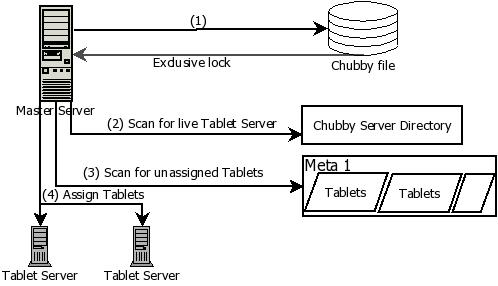
\includegraphics[width=5cm, height=5cm]{./figure/random.jpg}
	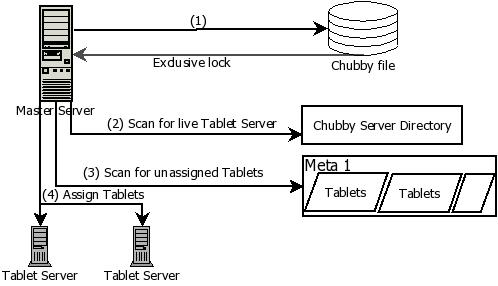
\includegraphics[width=.5\textwidth]{./figure/random.jpg}
	\caption{Random Pic}\label{f:random-pic}
\end{figure}


\begin{figure}

\begin{verbatim}
{     
    "firstName": "John"
    "lastName" : "Smith",
    "age" : 25
}
\end{verbatim}
\caption{JSON}
\end{figure}
